\section{Independence}

\definecolor{darkgreen}{rgb}{0,0.6,0}

\mode<presentation>{
\begin{frame} 
    \begin{center} \huge
        \secname
    \end{center}
    $$P(X,Y) = P(X)P(Y)$$
\end{frame}
}

\subsection{Motivation}

\begin{frame}\frametitle{\secname:~\subsecname}

The full joint distribution has everything we need to perform inference,
but it scales badly with more and more variables (e.g. adding $\mathit{Weather}$ (e.g. \# of weather conditions = 4) leads to a table with $2\times2\times2\times4=32$ entries)

\pause

\question{Should the weather be influenced by a $\mathit{cavity}$?}

\pause

\slidesonly{\vspace{-5mm}}

\begin{equation}
P(\mathit{cloudy} | \mathit{toothache}, \mathit{catch}, \mathit{cavity}) \stackrel{!}{=} P(\mathit{cloudy})
\end{equation}

\pause

\question{Should the weather have any influence on cavities, $\mathit{toothache}$ or the dentist?}

\pause

\notesonly{
-No, this independence can be formulated by:
}

\slidesonly{\vspace{-5mm}}

\begin{align}
P(\mathit{toothache}, \mathit{catch}, \mathit{cavity}, \mathit{Weather}) &\\
\stackrel{!}{=} P(\mathit{toothache}, &\mathit{catch}, \mathit{cavity})P(\mathit{Weather})
\end{align}


The 32 elements in the table can be split into \notesonly{the original} 8 + 4 \notesonly{(new table with 4 entries for the weather)}.

\end{frame} 

\begin{frame}\frametitle{\secname:~\subsecname}

``Extreme'' case:\\
 $n$ independent coin flips: $2^n$ combinations.\\
 Independence allows us to reduce this to $n \times$ single-variable distributions.

\end{frame}

\subsection{Bayes' theorem}

\mode<presentation>{
\begin{frame} 
    \begin{center} \huge
        \subsecname
    \end{center}
    
    \begin{equation*}
P(Y|X) = \frac{P(X|Y)P(Y)}{P(X)}
\end{equation*}
    
    \begin{center}   
   How do we get there? - product rule\\
     Why is it important? $\Rightarrow$ Conditional independence
    \end{center}
\end{frame}
}

\begin{frame}\frametitle{\subsecname}

Start with the product rule:

\begin{align}
P(X|Y)P(Y) = P(Y,X) &= P(X,Y) \visible<2->{= P(Y|X)P(X)\\
P(X|Y)P(Y) &= P(Y|X)P(X)}
\visible<3->{
\intertext{solve for $P(Y|X)$}
P(Y|X) = \frac{P(X|Y)P(Y)}{P(X)}
}
%\tag{Bayes' theorem}
\label{eq:bayes}
\end{align}

\end{frame}

\begin{frame}\frametitle{How to read Bayes' theorem}
\notesonly{
How to read Bayes' theorem:
}

\mode<presentation>{
    \begin{equation*}
P(Y|X) = \frac{P(X|Y)P(Y)}{P(X)}
\end{equation*}
}

\pause 

\only<2>{


\begin{figure}[h]
     \centering
	 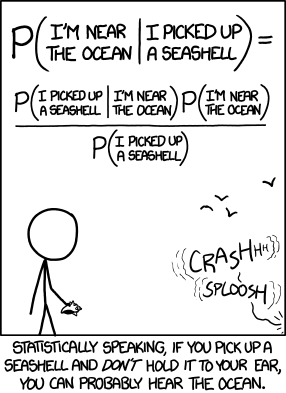
\includegraphics[width=0.33\textwidth]{img/xkcd_seashell}%
	 \caption{Bayes' Theorem example from \href{https://imgs.xkcd.com/comics/seashell.png}{xkcd.com}}
\end{figure}

}

\pause

\begin{equation}
\underbrace{P(\mathit{cause}|\mathit{effect})}_{\text{diagnositc}} = \frac{\overbrace{P(\mathit{effect}|\mathit{cause})}^{\text{causal}}P(\mathit{cause})}{P(\mathit{effect})}
\end{equation}

If $P(\mathit{effect})$ is missing, we can still normalize using:

\begin{equation}
P(Y|X) = \alpha P(X|Y)P(Y)
\end{equation}

$\alpha$ is chosen to whatever will make the entries in $P(Y|X)$ sum up to $1$.


\end{frame}

\subsection{Using Bayes' theorem}

\begin{frame}\frametitle{\subsecname}

\only<1>{
\begin{equation}
P(Y|X) = \alpha P(X|Y)P(Y)
\end{equation}

\begin{align}
P(\mathit{Cavity}|\mathit{toothache}=\text{true}, \mathit{catch}=\text{true}) &\\ 
=\alpha \underbrace{P(\mathit{toothache}=\text{true}, \mathit{catch}=\text{true}}_{\circledast} &| \mathit{Cavity})P(\mathit{Cavity})
\label{eq:applybayes}
\end{align}

$\circledast$ similar scaling problem, not much better then the case of using the full joint distribution.

}

\only<1,2>{

\question{Can we use independence to further mitigate the scaling problem here?}

}

\only<2>{

\begin{center}
$\mathit{Toothache}$ and $\mathit{Catch}$ are not independent.\\
But\\
$\mathit{Toothache}$ given $\mathit{cavity}$ is independent of $\mathit{Catch}$ given $\mathit{cavity}$
\end{center}

\begin{itemize}
\item $\mathit{toothache}$ depends on $\mathit{cavity}$: nerves \& tolerance for pain.
\item $\mathit{catch}$ depends on $\mathit{cavity}$: dependent on how skillful the dentist is.
\item \textbf{But}\ldots
\notesonly{``nerves \& tolerance for pain'' is \underline{independent} of ``how skillful the dentist is''.}
\end{itemize}

%TODO figure

}




\end{frame}

\begin{frame}

\mode<presentation>{
\slidesonly{\vspace{-5mm}
}

\begin{align}
P(\mathit{Cavity}|\mathit{toothache}=\text{true}, \mathit{catch}=\text{true}) &\\ 
=\alpha \underbrace{P(\mathit{toothache}=\text{true}, \mathit{catch}=\text{true}}_{\circledast} &| \mathit{Cavity}) P(\mathit{Cavity})
\label{eq:applybayes}
\end{align}

\begin{itemize}
\item $\mathit{toothache}$ depends on $\mathit{cavity}$: nerves \& tolerance for pain.
\item $\mathit{catch}$ depends on $\mathit{cavity}$: dependent on how skillful the dentist is.
\item \textbf{But}\ldots ``nerves \& tolerance for pain'' is \underline{independent} of ``how skillful the dentist is''.
\end{itemize}
}

Therefore:
\slidesonly{\vspace{-5mm}
}

\begin{align}
P(\mathit{toothache}
%=\text{true}
, \mathit{catch}
%=\text{true}
 | \mathit{Cavity}) &\\
= P(\mathit{toothache}
%=\text{true}
| \mathit{Cavity}) &P(\mathit{catch}
%=\text{true}
| \mathit{Cavity})
\label{eq:condindep}
\end{align}

i.e. \emph{conditional} independence of $\mathit{toothache}$ and $\mathit{catch}$ \underline{given} $\mathit{cavity}$

\pause

Plugging \eqref{eq:condindep} into \eqref{eq:applybayes} yields:

\slidesonly{\vspace{-4mm}}

\begin{align}
P(\mathit{toothache}, \mathit{catch} | \mathit{Cavity}) &\\
= \alpha P(\mathit{toothache}| \mathit{Cavity}) &
P(\mathit{catch}| \mathit{Cavity}) P(\mathit{Cavity})
\end{align}

i.e. \emph{conditional} independence of $\mathit{toothache}$ and $\mathit{catch}$ \underline{given} $\mathit{Cavity}$
\end{frame}

\subsection{Naive Bayes}

\begin{frame}\frametitle{\subsecname}

An alternate expression for the full joint distribution by exploiting conditional independence.

We start with the product rule:

\begin{equation}
P(X,Y) = P(X|Y)P(Y)    
\end{equation}

\begin{equation}
P(\mathit{Toothache},\mathit{Catch},\mathit{Cavity}) = P(\mathit{Toothache},\mathit{Catch}|\mathit{Cavity}) \underbrace{P(\mathit{Cavity})}_{\text{prior}} 
\end{equation}

Exploiting conditional independence yields:

\begin{align}
P(\mathit{Toothache},\mathit{Catch},\mathit{Cavity}) &\\
= P(\mathit{Toothache}|\mathit{Cavity}) &P(\mathit{Catch}|\mathit{Cavity}) \underbrace{P(\mathit{Cavity})}_{\text{prior}} 
\end{align}

\end{frame}

\begin{frame}\frametitle{\subsecname}

\mode<presentation>{
\begin{align*}
P(\mathit{Toothache},\mathit{Catch},\mathit{Cavity}) &\\
= P(\mathit{Toothache}|\mathit{Cavity}) &P(\mathit{Catch}|\mathit{Cavity}) \underbrace{P(\mathit{Cavity})}_{\text{prior}} 
\end{align*}
}

In terms of cause and effect:

\begin{align}
P(\mathit{Cause}, \mathit{Effect}_1, \mathit{Effect}_2,\ldots, \mathit{Effect}_n) &\\
= \underbrace{P(\mathit{Cause})}_{\text{prior}} &\prod_{i=1}^{n} P(\mathit{Effect}_{i}|\mathit{Cause})
\end{align}

Complexity reduced!

\end{frame}
